\chapter{SAT solvers}


\begin{description}
    \item[Satifiability (SAT)] \marginnote{SAT}
        Given a propositional formula $f$, 
        find an assignment of the variables to make the formula true.

        If $f$ is satisfiable, we say that it is SAT. Otherwise, it is UNSAT.
\end{description}

\begin{theorem}(Cook-Levin) \marginnote{Cook-Levin theorem}
    SAT is NP-complete.

    \begin{descriptionlist}
        \item[NP-complete]
            A problem is NP-complete iff it is in NP and every NP problem can be reduced to it.
            \begin{remark}
                All problems in NP can be reduced to SAT.
            \end{remark}
    \end{descriptionlist}
\end{theorem}


\begin{description}
    \item[Satisfiable formula] \marginnote{Satisfiable formula}
        A formula $f$ is satisfiable iff there is an assignment of the variables that makes it true.


    \item[Valid formula] \marginnote{Valid formula}
        A formula $f$ is valid iff any assignment of the variables makes it true.

        \begin{remark}
            $f$ is valid iff $\lnot f$ is UNSAT.
        \end{remark}


    \item[SAT solver] \marginnote{SAT solver}
        Given a problem, the following steps should be followed to solve it using a SAT solver:
        \begin{enumerate}
            \item Formalize the problem into a propositional formula.
            \item Depending on the solver, it might be necessary to convert in into CNF.
            \item Feed the formula to a SAT solver.
            \item The result can be an assignment of the variables (SAT) or a failure (UNSAT).
        \end{enumerate}
\end{description}



\section{Resolution}

\begin{description}
    \item[Resolution] \marginnote{Resolution}
        Basic approach for SAT.
        Prove that a set of CNF clauses is UNSAT by deriving new clauses until a contradiction is reached.

        Resolution rules to derive new clauses are:
        \begin{descriptionlist}
            \item[Resolution rule] \marginnote{Resolution rule} 
                \phantom{}
                \begin{minipage}{0.4\linewidth}
                    \begin{prooftree}
                        \AxiomC{$p \vee V$}
                        \AxiomC{$\lnot p \vee W$}
                        \BinaryInfC{$V \vee W$}
                    \end{prooftree}
                \end{minipage}

            \item[Unit resolution] \marginnote{Unit resolution}
                \begin{minipage}{0.4\linewidth}
                    \begin{prooftree}
                        \AxiomC{$p$}
                        \AxiomC{$\lnot p \vee W$}
                        \BinaryInfC{$W$}
                    \end{prooftree}
                \end{minipage}
                \begin{minipage}{0.4\linewidth}
                    \begin{prooftree}
                        \AxiomC{$\lnot p$}
                        \AxiomC{$p \vee V$}
                        \BinaryInfC{$V$}
                    \end{prooftree}
                \end{minipage}

                Note that this is equivalent to the rule of implication elimination:\\
                \begin{minipage}{0.4\linewidth}
                    \begin{prooftree}
                        \AxiomC{$p$}
                        \AxiomC{$p \Rightarrow W$}
                        \BinaryInfC{$W$}
                    \end{prooftree}
                \end{minipage}
                \begin{minipage}{0.4\linewidth}
                    \begin{prooftree}
                        \AxiomC{$\lnot p$}
                        \AxiomC{$\lnot p \Rightarrow V$}
                        \BinaryInfC{$V$}
                    \end{prooftree}
                \end{minipage}
        \end{descriptionlist}
\end{description}

\begin{example}
    Given the CNF formula:
    \[ (p \vee q) \land (\lnot r \vee s) \land (\lnot q \vee r) \land (\lnot r \vee \lnot s) \land (\lnot p \vee r) \]
    Resolution can be applied as follows:
    \begin{itemize}
        \item The starting clauses are:
            $(p \vee q) \cdot (\lnot r \vee s) \cdot (\lnot q \vee r) \cdot (\lnot r \vee \lnot s) \cdot (\lnot p \vee r)$
        \item From $(p \vee q)$ and $(\lnot q \vee r)$, one can derive $(p \vee r)$.
        \item From $(\lnot p \vee r)$ and $(p \vee r)$, one can derive $r$.
        \item From $(\lnot r \vee s)$ and $r$, one can derive $s$.
        \item From $(\lnot r \vee \lnot s)$ and $s$, one can derive $\lnot r$.
        \item From $r$ and $\lnot r$, one reaches $\bot$.
    \end{itemize}
\end{example}



\section{DPLL algorithm}

\begin{description}
    \item[DPLL] \marginnote{DPLL} 
        Algorithm based on unit resolution.
        Given a set of clauses, DPLL is applied as follows:
        \begin{enumerate}
            \item Apply unit resolution as long as possible 
                (i.e. for every clause containing a single literal $l$, remove $\lnot l$ from all clauses. 
                Clauses containing $l$ can also be removed as they are redundant).
            \item Choose a variable $p$.
            \item Recursively apply DPLL by assuming $p$ in one call and $\lnot p$ in another.
        \end{enumerate}

        \begin{theorem}
            DPLL is complete.
        \end{theorem}

        \begin{remark}
            DPLL efficiency strongly depends on the variables.
        \end{remark}
\end{description}

\begin{example}
    Given a CNF formula with clauses:
    \[ (\lnot p \vee \lnot s) \cdot (\lnot p \vee \lnot r) \cdot (\lnot q \vee \lnot t) \cdot (p \vee r) \cdot (p \vee s) \cdot (r \vee t) \cdot (\lnot s \vee t) \cdot (q \vee s) \]
    There are no unit clauses, so we choose the variable $p$ and consider the cases where $p$ and where $\lnot p$.

    By assuming $p$, unit resolution can be applied as follows:
    \begin{itemize}
        \item $p$ with $(\lnot p \vee \lnot s)$ derives $\lnot s$.
        \item $p$ with $(\lnot p \vee \lnot r)$ derives $\lnot r$.
        \item $\lnot s$ with $(q \vee s)$ derives $q$.
        \item $\lnot r$ with $(r \vee t)$ derives $t$.
        \item $q$ with $(\lnot q \vee \lnot t)$ derives $\not t$.
        \item $t$ and $\lnot t$ bring to $\bot$. This branch is UNSAT.
    \end{itemize}

    By assuming $\lnot p$, unit resolution can be applied as follows:
    \begin{itemize}
        \item $\lnot p$ with $(p \vee r)$ derives $r$.
        \item $\lnot p$ with $(p \vee s)$ derives $s$.
        \item $s$ with $(\lnot s \vee t)$ derives $t$.
        \item $t$ with $(\lnot q \vee \lnot t)$ derives $\lnot q$.
    \end{itemize}
    We reached a full assignment $\langle \lnot p, r, s, t, \lnot q \rangle$. The formula is SAT.
\end{example}

\begin{description}
    \item[DPLL implementation] \marginnote{DPLL algorithm}
        An efficient implementation of DPLL uses a list $M$ of the literals that have been decided or derived.

        \begin{description}
            \item[Notations] \phantom{}
                \begin{itemize}[leftmargin=*]
                    \item A literal $l$ holds in $M$ ($M \models l$) iff $l$ is in $M$.
                    \item $M$ contradicts a clause $C$ ($M \models \lnot C$) iff for every literal $l$ in $C$, $M \models \lnot l$.
                    \item A literal $l$ is undefined iff $M \cancel{\models} l$ and $M \cancel{\models} \lnot l$.
                    \item A decision literal (i.e. literal assumed to hold) is denoted as $l^\mathcal{D}$.
                \end{itemize}
        \end{description}

        The algorithm follows four rules:
        \begin{descriptionlist}
            \item[\texttt{UnitPropagate}] 
                If the CNF contains a clause $(A \vee l)$ such that $M \models \lnot A$ and $l$ is an undefined literal,
                then there is a transition:
                \[ M \rightarrow Ml \]

            \item[\texttt{Decide}] 
                When \texttt{UnitPropagate} it not possible, an undefined literal $l$ is assumed to hold (it becomes a decision literal):
                \[ M \rightarrow Ml^\mathcal{D} \]

            \item[\texttt{Backtrack}] 
                When a branch is UNSAT, the algorithm backtracks to the nearest decision literal and negates it.
                Given a clause $C$ of the CNF, if $Ml^\mathcal{D}N \models \lnot C$ and $N$ does not contain other decision literals,
                then there is a transition:
                \[ Ml^\mathcal{D}N \rightarrow M \lnot l \]

            \item[\texttt{Fail}] 
                Given a clause $C$ of the CNF, if $M \models \lnot C$ and $M$ contains a definitive assignment of all the variables (i.e. no decision literals),
                then there is a transition:
                \[ M \rightarrow \text{fail} \]
        \end{descriptionlist}

        In the end, if the formula is SAT, $M$ contains an assignment of the variables.
\end{description}

\begin{remark}
    Compared to resolution, DPLL is more memory efficient.
\end{remark}



\section{Conflict-driven clause learning (CDCL)}

DPLL with two improvements:
\begin{descriptionlist}
    \item[Clause learning] 
        When a contradiction is found, augment the original CNF with a conflict clause
        to prune the search space.

        The conflict clause is obtained through resolution by combining two clauses that cause the contradiction.

    \item[\texttt{Backjumping}]
        Depending on the type of contradiction, skip decision literals that are not causing the conflict
        and directly backtrack to an earlier relevant decision literal.

        Given a clause $C$ of the CNF, if $Ml^\mathcal{D}N \models \lnot C$ and 
        there is a clause $(C' \vee l')$ derivable from the CNF such that $M \models \lnot C'$ and
        $l'$ is undefined, then there is a transition:
        \[ Ml^\mathcal{D}N \rightarrow Ml' \] 
        Note that $N$ might contain other decision literals and $(C' \vee l')$ is a conflict clause.

        \begin{remark}
            \texttt{Backjumping} can be seen as \texttt{UnitPropagate} applied on conflict clauses.
        \end{remark}
\end{descriptionlist}

\begin{description}
    \item[Implication graph]
        DAG $G=(V, E)$ to record the history of decisions and unit resolutions.
        \begin{descriptionlist}
            \item[Vertex] Can be:
                \begin{itemize}
                    \item A decision or derived literal (denoted as $l@d$, where $l$ is the literal and $d$ the decision level it originated from).
                    \item A marker to indicate a conflict (denoted as $\kappa@d$, where $d$ is the decision level it originated from).
                \end{itemize}

            \item[Edge] 
                Has form $v \xrightarrow{c_i} w$ and indicates that $w$ is obtained using the clause $c_i$ and the literal $v$.
        \end{descriptionlist}
        
        \begin{example}
            Starting from the clauses $c_1, \dots, c_6$ of a CNF, one can build the implication graph while running DPLL/CDCL.

            In this example, the decision literals (green nodes) are assigned following this order: $x_1 \rightarrow x_8 \rightarrow \lnot x_7$:
            \begin{center}
                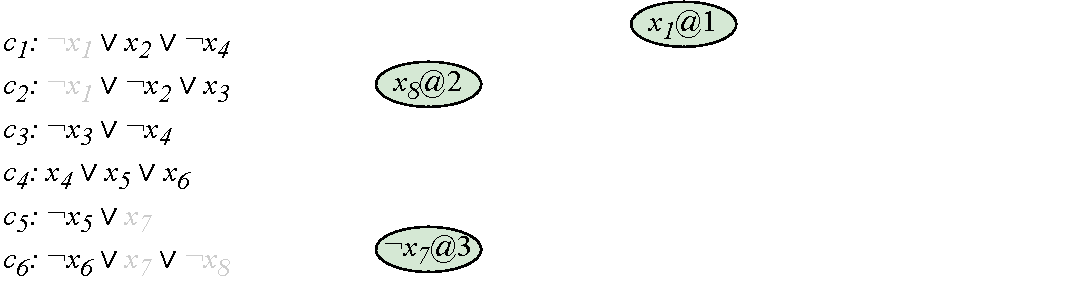
\includegraphics[width=0.8\linewidth]{./img/_cdcl_example1.pdf}
            \end{center}
            \[ M \rightarrow M x_1^\mathcal{D} x_8^\mathcal{D} \lnot x_7^\mathcal{D} \]

            Then, it is possible to derive implied variables using unit resolution starting from the decision literals:
            \begin{center}
                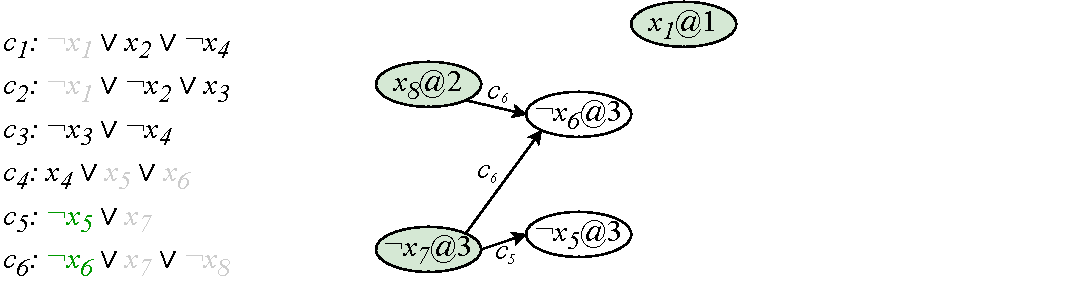
\includegraphics[width=0.8\linewidth]{./img/_cdcl_example2.pdf}
            \end{center}
            \[ M \rightarrow M \lnot x_6 \lnot x_5 \]
            And so on:
            \begin{center}
                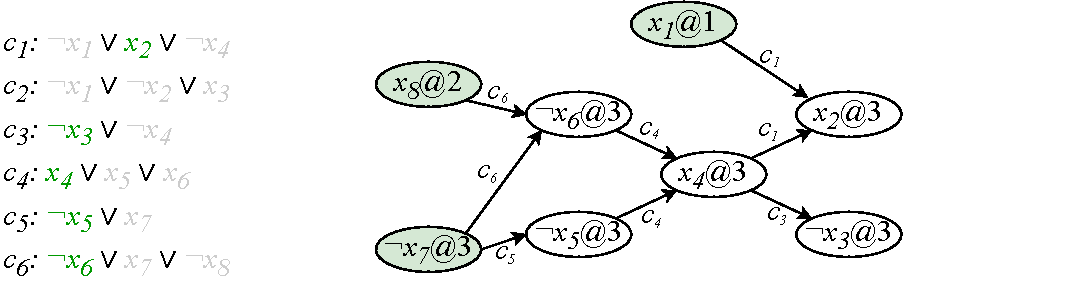
\includegraphics[width=0.8\linewidth]{./img/_cdcl_example3.pdf}
            \end{center}
            \[ M \rightarrow M x_4 x_2 \lnot x_3 \]

            As $c_2$ is UNSAT, we reached a contradiction:
            \begin{center}
                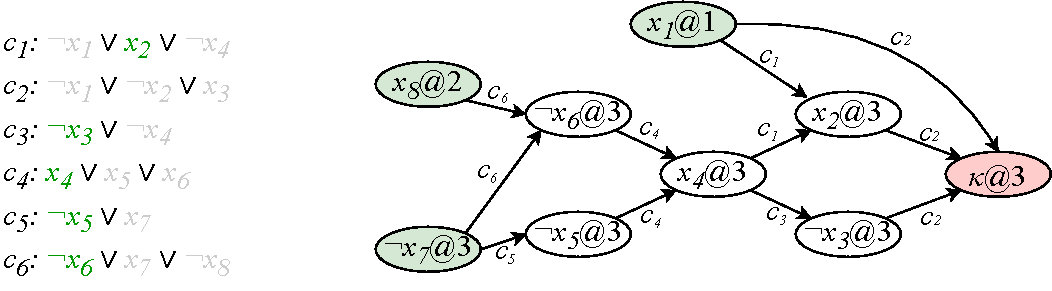
\includegraphics[width=0.8\linewidth]{./img/_cdcl_example4.pdf}
            \end{center}
        \end{example}

    \begin{remark}
        Any cut that separates sources (decision literals) and the sink (contradiction node) is a valid conflict clause for backjumping.

        \begin{example} \phantom{}
            \begin{center}
                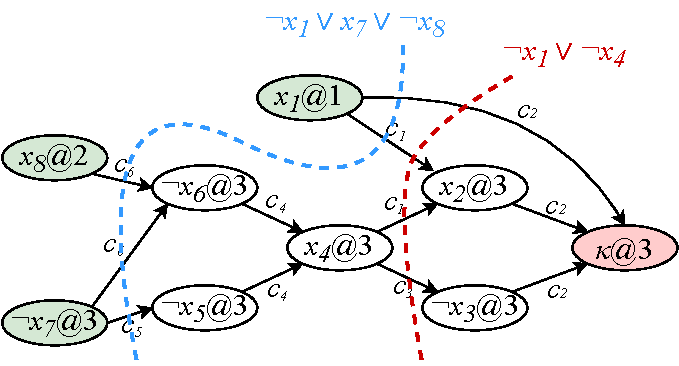
\includegraphics[width=0.55\linewidth]{./img/_cdcl_cut.pdf}
            \end{center}
        \end{example}
    \end{remark}

    \item[Unit implication point (UIP)]
        Given an implication graph where the latest decision node is $(l@d)$ and the conflict node is $(\kappa@d)$,
        a node is a unit implication point iff it appears in all the paths from $(l@d)$ to $(\kappa@d)$.

        The UIP closest to the conflict is denoted as 1UIP.

        \begin{remark}
            The decision node $(l@d)$ itself is a UIP.
        \end{remark}

    \item[1UIP-based backjumping]
        In case of conflict, use the conflict clause obtained by cutting in front of the 1UIP.

        \begin{remark}
            This allows to:
            \begin{itemize}
                \item Reduce the size of the conflict clause.
                \item Guarantee the highest backtrack jump.
            \end{itemize}
        \end{remark}

        \begin{example}
            \phantom{}
            \begin{center}
                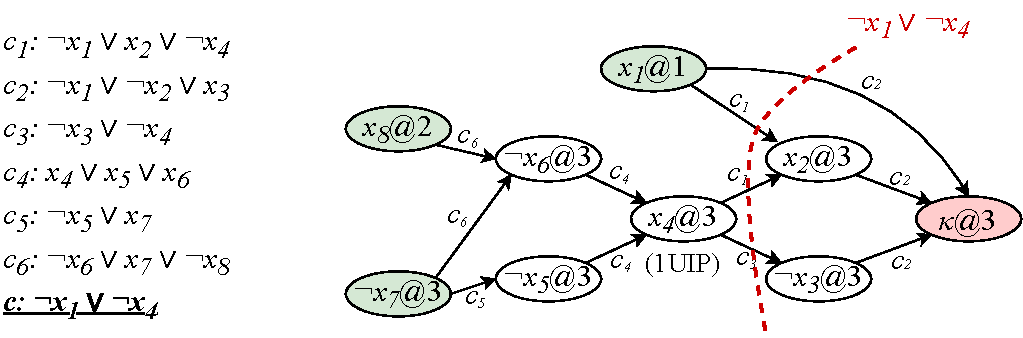
\includegraphics[width=0.75\linewidth]{./img/_cdcl_1uip.pdf}
            \end{center}
            By adding the conflict clause $(\lnot x_1 \vee \lnot x_4)$, we can backjump up to $x_8^\mathcal{D}$ 
            (not to $x_1^\mathcal{D}$ as it makes the conflict clause a unit).
            \[ x_1^\mathcal{D} x_8^\mathcal{D} \lnot x_7^\mathcal{D} \lnot x_6 \lnot x_5 x_4 x_2 \lnot x_3 \rightarrow x_1^\mathcal{D} \lnot x_4\]
        \end{example}
\end{description}